Following the design phase, it is crucial to test the protocol in a practical environment in order to verify that it works as intended. Furthermore,
extensive performance evaluations need to be conducted to assure the viability of the devised techniques. Both of these tasks are achieved through
thorough software simulation. For this purpose, a dedicated, cycle-accurate simulator was developed that supports the designed protocol with all the
features described in Chapter \ref{ch:protocol}. A very small portion of the codebase was already implemented before this thesis at the TU Dresden
Chair of Privacy and Data Security. However, most of it was refactored and the vast majority of the source code was written from scratch.

The simulator is implemented in C++ and based on the \textit{\omnet{}} discrete event simulation framework \cite{omnet}. \omnet{} provides a general-purpose
network simulation architecture and promotes a modular design. In general, it allows the programmer to define the components of the network via a
special scripting language called \textit{NED}. With NED files, modules may be specified as they appear from the outside, by means of parameters,
gates, and connections. Furthermore, a module is allowed to have any number of submodules, facilitating a hierarchical structure. A C++
class is assigned to each module that controls the component's internal behavior together with the parameters. The gates define the ports of the
module through which it sends and receives messages. The connections link the gates of different modules (or submodules) together and thus define the
message flows and the network's topology.

The simulator makes extensive use of the hierarchical and modular approach of \omnet{}. The processing elements, network interfaces, and routers are
defined as modules and instanced as many times as required, depending on the \gls{noc} dimensions. They are interconnected through their gates and
arranged in a way mirroring the structure of the \gls{noc}. To create a simulation as realistic as possible, they are made up of a number of
submodules, such as queues, buffers, and crypto modules, resembling the actual hardware layout.

\omnet{} allows the user to freely implement detailed statistics to be recorded during simulations. They provide the foundation for the evaluation
in Chapter \ref{ch:evaluation}. Data sets are obtained by running numerous simulations with varying configurations.

In Section \ref{sec:generalass}, fundamental assumptions about the simulation environment are presented. Subsequently, Section
\ref{sec:componentstructure} elaborates on the hierarchical structure of the components and their layout. Finally, an overview of the internal delays
and latencies that the various submodules entail is given in Section \ref{sec:internaldelays}.

\section{General Assumptions}\label{sec:generalass}
\subsection{The GALS Paradigm}
In Section \ref{sec:networkonchipfun}, it was mentioned that \glspl{noc} lend themselves well to the implementation of the \gls{gals} design paradigm.
For the simulation, it was not considered for three reasons. First, its usage requires the existance of multiple clock domains: each core runs with the
frequency best suited for itself and is not synchronized with other cores in the network (\enquote{globally asynchronous}). This, however, is very
finical to implement correctly. Second, since the cores themselves each operate under a single clock (\enquote{locally synchronous}), \gls{gals} would
only affect the transmissions from one router to another. Third, the cores are assumed to be identical and hence run with the same frequency anyway.
On these grounds, a globally synchronous architecture with a single clock driving all components is used in the simulator.

\subsection{Clock Frequency}
The \gls{noc}'s global clock runs at a frequency of 500 MHz as this is a common speed in \gls{noc}-related research
\cites{frey15stateobfuscation}{frey17hardenednoc}. Unfortunately, the PRINCE cipher that is employed for all cryptographic operations is unable to run at
such a high frequency. However, in Section \ref{subsubsec:prince} it was shown that the algorithm runs flawlessly at frequencies of up to 250 MHz.
Thus, the crypto modules operate at half the frequency of the \gls{noc}, with every two cycles of the global clock corresponding to one
cycle for the crypto modules. Hence, the processing of a single block with PRINCE is assumed to take two clock cycles in the simulator.

It was mentioned above that the integration of multiple clock domains is very finical. However, when they are not independent and the global clock's
frequency is evenly divisible by the required frequency, as is the case for the crypto modules, this becomes significantly easier. Here, a new clock
is derived from the global clock that simply omits every other tick.

\subsection{Single Cycle Routing}
The number of cycles required for routing\footnote{Routing refers to the whole process from receiving a flit on an input port to forwarding it on the
appropriate output port, including route calculation, switch allocation, and switch traversal \cite[see][2]{routinglectureutah}.} is a key factor to the
overall performance of the \gls{noc}. While four cycle \cite[e.g.][]{routinglectureutah} and two cycle routing \cite[e.g.][]{lu11nocrouter} are
popular approaches, architectures requiring only a single cycle have also proven to be both feasible and practical
\cites{hayenga09scarab}{ved17routeonfly}.

As achieving low latencies is of utmost importance for this thesis, single cycle routing is implemented in the simulator. Such an approach is easily
able to operate at the required frequency of 500 MHz \cite[7]{hayenga09scarab}. Furthermore, high routing speeds imply less required buffers
\cite[1]{ved17routeonfly}, reducing the occupied chip area of the routers. Although completely bufferless architectures are possible
\cite{hayenga09scarab}, the implemented scheme grants each router one input buffer per port (i.e., five buffers per router) in order to prevent
immediate discarding of flits in the case of link congestions. Output buffers, however, are not used.

In order for the complexity of the simulator to stay within manageable bounds, the internal structure of the routers is kept simple. For instance, no
virtual channels are used for the input buffers mentioned above. This, however, implies that a flit delayed by a congestion of the targeted output
link also holds back all following flits in the buffer, even if they would be routed to a different link.

\subsection{Retransmission Buffer}
In Section \ref{subsec:arqretransmissions}, it was mentioned that \glspl{arq} are not authenticated. This implies that there is no method to ensure
the integrity of \glspl{arq}. However, the worst case scenario is that a modified \gls{arq} causes different flits to be retransmitted than the
intended ones, entailing unnecessary network load. To simplify this case, a modified \gls{arq} is ignored by the \gls{rtb}.

\section{Component Structure}\label{sec:componentstructure}
This section provides an in-depth view on the modular structure of the simulator. In a top-down approach, it begins with the outermost layer of the
hierarchy (i.e., the \gls{noc} itself) and then descends into the individual components. The figures used to support the textual explanations are
drawn directly from the graphical interface provided by \omnet{}.

\subsection{Complete Network}
The structure of the \gls{noc} in the simulator mirrors the 2D mesh topology of the network (cf. Figure \ref{fig:nocexample}). The only difference
here is that the network interfaces are not built as submodules of the processing elements, but as independent components interposed between the
processing elements and routers. Figure \vref{fig:omnetnoc} visualizes this approach.

\begin{figure}
    \centering
    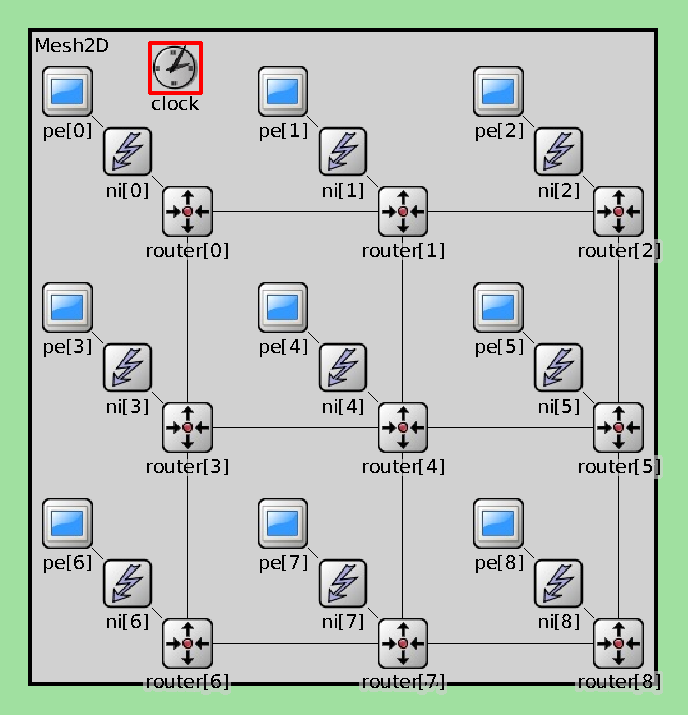
\includegraphics[width=0.5\textwidth]{omnet-noc}
    \caption[Simulator view of the NoC]{The \gls{noc} as it appears in \omnet{}. For clarity reasons, it was truncated to a 3x3 mesh. Each processing
    element, network interface, and router are assigned an index for simulation purposes. The network interfaces were not integrated into the
    processing elements to allow for better visualizations of the traffic flow.}
    \label{fig:omnetnoc}
\end{figure}

In addition to these familiar components, the global clock is also implemented as its own module. As a part of the simulation, it drives all other
modules and their submodules through signals. Any module may attach itself to this clock by registering as a receiver for the appropriate signal.

\subsection{Processing Element}
The processing element is a very plain component from the perspective of the simulator. It contains nothing more than a traffic generator and a flit
consumer with an input queue. Figure \vref{fig:omnetpe} depicts its appearance in \omnet{}.

\begin{figure}
    \centering
    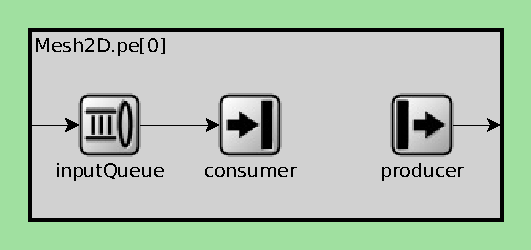
\includegraphics[width=0.5\textwidth]{omnet-pe}
    \caption[Simulator view of the processing element]{An instance of a processing element module of \omnet{}. A traffic generator (producer) randomly
    creates flits and sends them to the connected network interface. Flits arriving from the network interface are accepted by a pseudo-buffer
    (inputQueue) that subsequently passes them to the consumer.}
    \label{fig:omnetpe}
\end{figure}

The traffic generator randomly produces flits and sends them to the network interface. On each clock tick, one flit is created with a configurable
\textit{generation probability}. The destination is chosen at random from the set of network nodes (excluding the own node) with a uniform
distribution. The produced flits are always data flits (not \glspl{mac} or \glspl{arq}) without any meaningful information contained in their
payloads\footnote{For the simulation, only the transmission parameters are of interest, not the actual data being transferred.}. Furthermore, the
generator may be configured to always produce a pair of two flits: in the event of a flit creation as described above, another flit will always be
produced on the next clock tick with the same destination. The purpose of this generation pattern is to allow for a fair comparison of uncoded and
network coded protocol variants and explained in detail in Section (insert ref here).

The flit consumer simply accepts any flits arriving from the local network interface and records these events with \omnet{}'s statistics system. Since
the flits are of no further use after this, they are subsequently destroyed. An input buffer is located in front of the consumer to ensure both
synchronization with the global clock and that the travel time from network interface to processing element is precisely one cycle.

\subsection{Network Interface}
The network interface is the most complex part of the simulator. Implementing all the logic required by the protocol, it contains several crypto
modules, network coding components, the retransmission buffer as well as the verification and \gls{arq} infrastructure. The layout of these components
slightly differs for each variant. However, all variants resemble the structure of their corresponding flowchart in Section \ref{sec:theprotocol}, so
explaining the network interface by means of one variant is deemed sufficient. For this purpose, the network coded interwoven authentication version
is described below. Figure \vref{fig:omnetni} shows the internal structure as rendered by \omnet{}'s graphical interface.

\begin{figure}
    \centering
    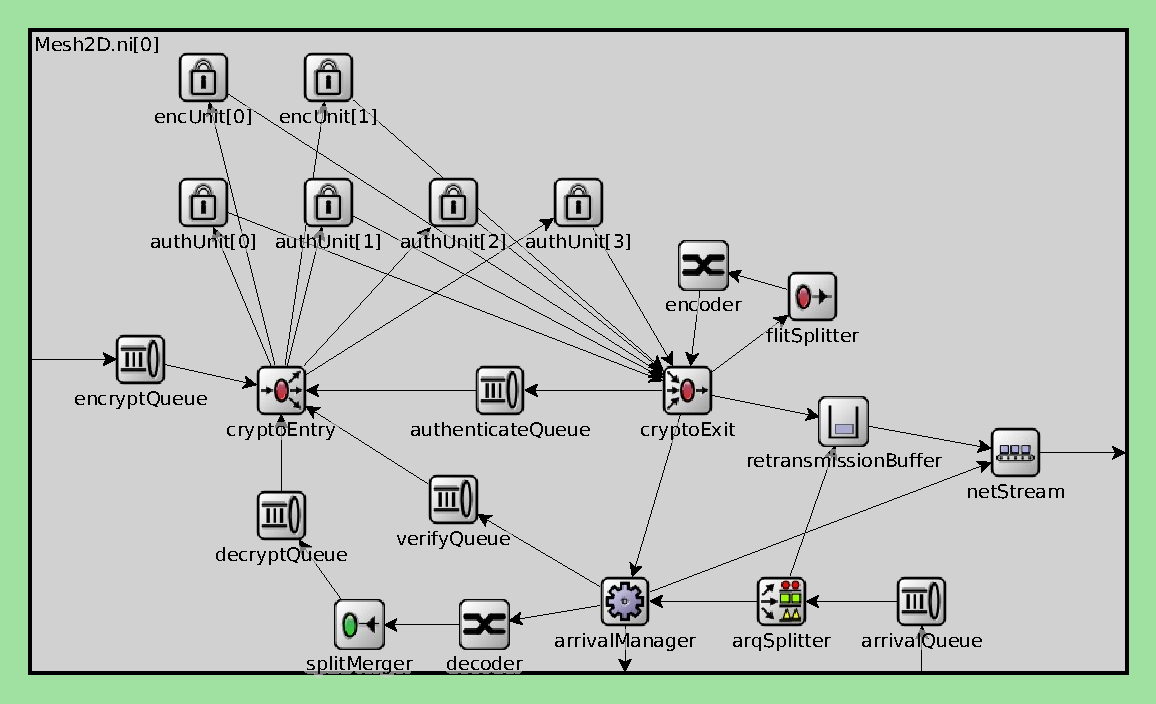
\includegraphics[width=0.85\textwidth]{omnet-ni}
    \caption[Simulator view of the network interface]{An instance of a network interface for network coded interwoven authentication as rendered by
    \omnet{}. Flits from the processing element arrive on the left side and subsequently traverse a pipeline of encryption, encoding, and
    authentication modules. The flits from the router enter the interface on the bottom right. After \glspl{arq} are filtered out, the remaining flits
    are subjected to decoding, decryption, and verification procedures before being forwarded to the processing element.}
    \label{fig:omnetni}
\end{figure}

The network interface was modeled as accurately as possible to facilitate detailed statistics about the flit flow inside them. This allows for the
evaluation of internal delays that are caused, for instance, by departing and arriving flits competing over the available crypto modules, or a
retransmission competing with a new flit over the link to the router. Thus, the implementation of the network interfaces consists of a number of
different submodules, and flits take rather intricate paths through them. In the following sections, the progression of an exemplary transmission unit
both for departing (\gls{pe} $\rightarrow$ router) and arriving (router $\rightarrow$ \gls{pe}) flits is given.

\subsubsection{Path Of Departing Flits}
Flits entering the network interface from the processing element are first placed into a queue (\textit{encryptQueue} module on the left side of
Figure \ref{fig:omnetni}). As the name suggests, they wait here for an encryption module to become available. Once this is the case, the front
flit is fetched from the queue and redirected to the appropriate encryption module.

The network interface's crypto modules are managed by an auxiliary module (named \textit{cryptoEntry} in Figure \ref{fig:omnetni}). It keeps track of
the availability status of both the encryption and the authentication modules and handles the distribution of flits among them. There are multiple
queues connected to it; the aforementioned \textit{encryptQueue} and three others whose role will be explained below. It should be noted that only one
flit can be fetched from each queue per clock cycle. In the current path of the exemplary flit, \textit{cryptoEntry} will fetch it from
\textit{encryptQueue} once one of the encryption modules (named \textit{encUnit} suffixed with an index in Figure \ref{fig:omnetni}) becomes
available.

Once the encryption module has finished its task, the flit arrives at another auxiliary module where the paths from all crypto modules converge.
Aptly named \textit{cryptoExit} in Figure \ref{fig:omnetni}, incoming flits are redirected depending on their arrival gate. For the current case, the
encrypted flit is sent to the \textit{flitSplitter}.

With the interwoven authentication protocol variant, the next step is to create a new flit that half the payload is moved to. Afterwards, these two
flits are encoded as a generation by the \textit{encoder}. The resulting three or four flits are subsequently sent back to the \textit{cryptoExit}
auxiliary module which merely forwards them to the \textit{authenticateQueue}. As the computation of a combination takes one clock cycle, the encoder
consequently sends out precisely one combination per cycle.

Now, each combination needs to be authenticated. The \textit{authenticateQueue} is one of the four queues connected to the \textit{cryptoEntry}. In
the same manner as for the encryption process, \textit{cryptoEntry} fetches the front flit from the \textit{authenticateQueue} once one of the
authentication modules (referred to as \textit{authUnit} suffixed with an index in Figure \ref{fig:omnetni}) is available and forwards it
appropriately.

When the authentication process is complete, the flits once again arrive at the \textit{cryptoExit}. This time, however, they are forwarded to the
\textit{retransmissionBuffer}. Here, each one is copied as specified in the protocol before being sent to the network. The \textit{netStream} is
another auxiliary module that merely serializes departing flits, retransmissions, and issued \glspl{arq} in case they arrive here at the same clock
cycle. This is necessary since multiple flits cannot occupy the link to the router at the same time.

\subsubsection{Path Of Arriving Flits}
When a flit arrives from the network, it is first placed into a queue (named \textit{arrivalQueue} and located at the bottom right of Figure
\ref{fig:omnetni}). However, flits are only kept here until the next clock tick. The purpose of this procedure is to ensure that the travel time from
the router was precisely one clock cycle.

The next station is the \textit{arqSplitter} supplementary module. Its only task is to check the incoming flit's mode field. In case of an
\gls{arq}, it is sent straight to the \textit{retransmissionBuffer} which subsequently performs the appropriate retransmissions. Otherwise, the flit
is forwarded to the \textit{arrivalManager}.

The \textit{arrivalManager} is the most complex submodule of the network interface. It buffers incoming flits, performs verifications through authcode
comparisons, and keeps track of the \gls{arq} timeouts for all the transmission units. For each arriving flit, two copies are made: one to compute an
authcode over and one for decoding and decryption.

While the original is stored for the upcoming verification process, the first copy is sent to the
\textit{verifyQueue}, which is connected to the \textit{cryptoEntry}. Identically to the departing flits waiting for authentication, the
\textit{cryptoEntry} fetches flits from the queue once an authentication module is available. However, in case there are flits in both the
\textit{authenticateQueue} and the \textit{verifyQueue}, the former always takes priority\footnote{The rationale for preferring departing flits is to
not disperse generations that will be sent to the network. If the flits are already spaced out when leaving the interface, the probability for causing
unnecessary \gls{arq} timeouts increases needlessly.}.

The second copy is forwarded to the decoder. It is buffered here until another flit from the
same transmission unit arrives. Both are subsequently decoded and merged back into a single flit, which is then sent to the \textit{decryptQueue}. As
the name suggests, the flit stands by until the \textit{cryptoEntry} has allocated an encryption module for it\footnote{As laid out in Section
\ref{subsubsec:prince}, the encryption modules are able to perform decryptions as well.}. Corresponding to the authentication process, departing flits
take priority over the encryption module access when both \textit{decryptQueue} and \textit{encryptQueue} are not empty. Both the decrypted flits and
computed authcodes are redirected back to the \textit{arrivalManager} by the \textit{cryptoExit}. Authcodes are compared with those contained in the
originally buffered flits; in case of their equality, the decrypted flit is sent directly to the processing element.

In case an \gls{arq} must be issued, either caused by non-equal authcodes or timeouts, the \textit{arrivalManager} generates and prepares an
\gls{arq} flit. From there, it is sent to the network via the \textit{netStream} auxiliary serialization module.

\subsection{Router}\label{subsec:routerimpl}
Like the processing elements, the routers' internal structure is straightforward. Presented in Figure \vref{fig:omnetrouter}, it consists of a switch
and five input buffers (one for the local network interface and four for the neighboring routers).

\begin{figure}
    \centering
    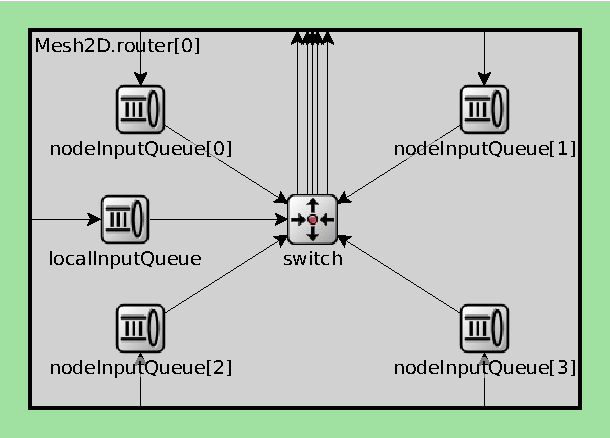
\includegraphics[width=0.55\textwidth]{omnet-router}
    \caption[Simulator view of the router]{An instance of a router as rendered by \omnet{}. The five input gates are connected to the switch via their
    input queues. The five respective output connections are not interposed by a buffer. In the renderings of \omnet{}, the spatial layout of the
    connections sometimes does not match their logical correlations, as is the case here with the output lines being drawn in parallel. However, there is
    in fact one output connection corresponding to each input gate.}
    \label{fig:omnetrouter}
\end{figure}

The routing logic is located within the switch submodule. On every clock tick, it checks the front flits in each queue and computes the most suitable
output ports for them. This computation (often referred to as \textit{route calculation}) depends on the flit's destination header and the implemented routing
strategy. If a calculated output port is unavailable due to the link being congested, the affected flits are delayed until the next clock tick.
Furthermore, in case multiple flits are to be routed through the same output port, one of them is randomly selected while the others are postponed.
Flits from different queues with differing output ports can be routed simultaneously.

Routers are able to inform neighboring ones of congestions of their input queues. Once a queue is full, the router sends a congestion signal to the
neighbor connected to this queue\footnote{For instance, these notifications can be realized through dedicated signaling lines on the router
interconnections. This would increase the channel width from 141 to 142 wires or from 149 to 150 wires for uncoded and network coded protocols,
respectively (cf. Section \ref{subsec:flitstructure}).}, thereby instructing it to delay all flits that are supposed to be routed towards the
signaling router. Once the congestion has subsided, the affected neighbor is informed of this event through a similar signal and may resume the
routing of flits in the affected direction normally.

\section{Internal Delays}\label{sec:internaldelays}
To provide a better understanding of the impact of each module on the overall processing latency, their delays are given in a concise, tabular form.
Table \ref{tab:processinglatencies} presents the processing times for the submodules of the network interfaces, while Table
\vref{tab:transmissionlatencies} shows the transmission durations between the \gls{noc}'s components.

\begin{table}
    \centering
    \begin{tabulary}{\textwidth}{R|L}
        Procedure & Delay in cycles \\\hline
        Encryption/decryption & 2 \\
        Encoding (G2C3) & 3 (1 per combination) \\
        Encoding (G2C4) & 4 (1 per combination) \\
        Authentication (individual) & 6 \\
        Authentication (interwoven) & 5 \\
        Authentication (full gen.) & 10 \\
        Decoding & 2 (1 per flit) \\
        \gls{mac} comparison & 1 \\
        \gls{arq} composition & 1 \\
        Flit storage in \gls{rtb} & 1 \\
        \Gls{rtb} lookup & 1 (uncoded), 2 (network coded)
    \end{tabulary}
    \caption[Internal computation delay in the network interface]{Internal computation delays of various procedures within the network interfaces.}
    \label{tab:processinglatencies}
\end{table}

\begin{table}
    \centering
    \begin{tabulary}{\textwidth}{R|L}
        Transmission & Delay in cycles \\\hline
        PE $\Leftrightarrow$ NI & 1 \\
        NI $\Leftrightarrow$ Router & 1 \\
        Router $\Leftrightarrow$ Router & 1
    \end{tabulary}
    \caption[Transmission latencies for the NoC interconnections]{Transmission latencies of the \gls{noc} interconnections. The inter-router
    communication includes the route calculation and switching process in the originating router.}
    \label{tab:transmissionlatencies}
\end{table}

The delay for the encryption and decryption is precisely two clock cycles for all protocol variants a exactly one input block (the flit payload)
needs to be processed. For authentication, the number of input blocks (and consequently the delay) varies. With individual authentication, three
blocks are processed, corresponding to six clock cycles. Interwoven authentication only has two input blocks, but entails an additional cycle for the
authcode calculation. With full-generation authentication, the two input flits are divided into five blocks and thus require ten cycles of
processing.

The lookup procedure for the retransmission buffer works as follows: when an \gls{arq} arrives, the first action is to find the correct buffer
depending on the \gls{arq}'s source. As the location of each buffer is static, this does not require a dedicated clock cycle. Afterwards, the position
of the affected transmission unit inside the buffer needs to be identified by searching for the unit's ID, which takes one cycle. Finally, the
required flits are retrieved from the buffer using the modes specified in the \gls{arq}. Once the transmission unit's location is known, the position
of the individual flits is determined by fixed offsets from this location depending on the mode, which eliminates the need to search for each one.

Thus, for uncoded protocol variants, an \gls{rtb} lookup takes one clock cycle. However, if multiple flits need to be retransmitted, only one can be
sent out per cycle since the link to the router cannot be occupied by more than one flit at the same time.

In network coded environments, the mode header field does not suffice to uniquely identify a flit within a transmission unit; the \glspl{gev}
specified in the \gls{arq} need to be compared as well. Hence, a flit's position is determined by first finding the ID, then the affected \glspl{gev},
and finally the required modes for each \gls{gev}. This extended procedure adds one clock cycle to the lookup time for a total of two cycles.
